%%
%% This is file `sample-sigconf.tex',
%% generated with the docstrip utility.
%%
%% The original source files were:
%%
%% samples.dtx  (with options: `all,proceedings,bibtex,sigconf')
%% 
%% IMPORTANT NOTICE:
%% 
%% For the copyright see the source file.
%% 
%% Any modified versions of this file must be renamed
%% with new filenames distinct from sample-sigconf.tex.
%% 
%% For distribution of the original source see the terms
%% for copying and modification in the file samples.dtx.
%% 
%% This generated file may be distributed as long as the
%% original source files, as listed above, are part of the
%% same distribution. (The sources need not necessarily be
%% in the same archive or directory.)
%%
%%
%% Commands for TeXCount
%TC:macro \cite [option:text,text]
%TC:macro \citep [option:text,text]
%TC:macro \citet [option:text,text]
%TC:envir table 0 1
%TC:envir table* 0 1
%TC:envir tabular [ignore] word
%TC:envir displaymath 0 word
%TC:envir math 0 word
%TC:envir comment 0 0
%%
%%
%% The first command in your LaTeX source must be the \documentclass
%% command.
%%
%% For submission and review of your manuscript please change the
%% command to \documentclass[manuscript, screen, review]{acmart}.
%%
%% When submitting camera ready or to TAPS, please change the command
%% to \documentclass[sigconf]{acmart} or whichever template is required
%% for your publication.
%%
%%
\documentclass[sigconf]{acmart}

%%
%% \BibTeX command to typeset BibTeX logo in the docs
\AtBeginDocument{%
  \providecommand\BibTeX{{%
    Bib\TeX}}}

%% Rights management information.  This information is sent to you
%% when you complete the rights form.  These commands have SAMPLE
%% values in them; it is your responsibility as an author to replace
%% the commands and values with those provided to you when you
%% complete the rights form.
\setcopyright{none}
\copyrightyear{2024}
\acmYear{2024}
\acmDOI{XXXXXXX.XXXXXXX}

%% These commands are for a PROCEEDINGS abstract or paper.
\acmConference[COMP 5117]{Mining Software Repositories}{December 2024}{Ottawa, ON}
%%
%%  Uncomment \acmBooktitle if the title of the proceedings is different
%%  from ``Proceedings of ...''!
%%
\acmBooktitle{Mining Software Repositories, December 2024, Ottawa, ON}
\acmISBN{XXX-X-XXXX-XXXX-X/24/12}


%%
%% Submission ID.
%% Use this when submitting an article to a sponsored event. You'll
%% receive a unique submission ID from the organizers
%% of the event, and this ID should be used as the parameter to this command.
%%\acmSubmissionID{123-A56-BU3}

%%
%% For managing citations, it is recommended to use bibliography
%% files in BibTeX format.
%%
%% You can then either use BibTeX with the ACM-Reference-Format style,
%% or BibLaTeX with the acmnumeric or acmauthoryear sytles, that include
%% support for advanced citation of software artefact from the
%% biblatex-software package, also separately available on CTAN.
%%
%% Look at the sample-*-biblatex.tex files for templates showcasing
%% the biblatex styles.
%%

%%
%% The majority of ACM publications use numbered citations and
%% references.  The command \citestyle{authoryear} switches to the
%% "author year" style.
%%
%% If you are preparing content for an event
%% sponsored by ACM SIGGRAPH, you must use the "author year" style of
%% citations and references.
%% Uncommenting
%% the next command will enable that style.
%%\citestyle{acmauthoryear}


%%
%% end of the preamble, start of the body of the document source.
\begin{document}

%%
%% The "title" command has an optional parameter,
%% allowing the author to define a "short title" to be used in page headers.
\title{Assessing CodePilot's Breadth}

%%
%% The "author" command and its associated commands are used to define
%% the authors and their affiliations.
%% Of note is the shared affiliation of the first two authors, and the
%% "authornote" and "authornotemark" commands
%% used to denote shared contribution to the research.
\author{Justin Zhang}
\authornote{Both authors contributed equally to this research.}
\email{JustinZhang@cmail.carleton.ca}
\affiliation{
	\institution{Carleton University}
	\city{Ottawa}
	\state{Ontario}
	\country{Canada}
}
\author{Kaya Gouin}
\authornotemark[1]
\email{KayaGouin@cmail.carleton.ca}
\affiliation{
	\institution{Carleton University}
	\city{Ottawa}
	\state{Ontario}
	\country{Canada}
}

%%
%% By default, the full list of authors will be used in the page
%% headers. Often, this list is too long, and will overlap
%% other information printed in the page headers. This command allows
%% the author to define a more concise list
%% of authors' names for this purpose.
%\renewcommand{\shortauthors}{Trovato et al.}

%%
%% The abstract is a short summary of the work to be presented in the
%% article.
\begin{abstract}
	...
\end{abstract}

%%
%% The code below is generated by the tool at http://dl.acm.org/ccs.cfm.
%% Please copy and paste the code instead of the example below.
%%
\begin{CCSXML}
	<ccs2012>
	<concept>
	<concept_id>10011007</concept_id>
	<concept_desc>Software and its engineering</concept_desc>
	<concept_significance>300</concept_significance>
	</concept>
	</ccs2012>
	\ccsdesc[300]{Software and its engineering}
\end{CCSXML}

%%
%% Keywords. The author(s) should pick words that accurately describe
%% the work being presented. Separate the keywords with commas.
\keywords{Software engineering, prompt engineering, artificial intelligence, few-shot}
%% A "teaser" image appears between the author and affiliation
%% information and the body of the document, and typically spans the
%% page.
\iffalse
	\begin{teaserfigure}
		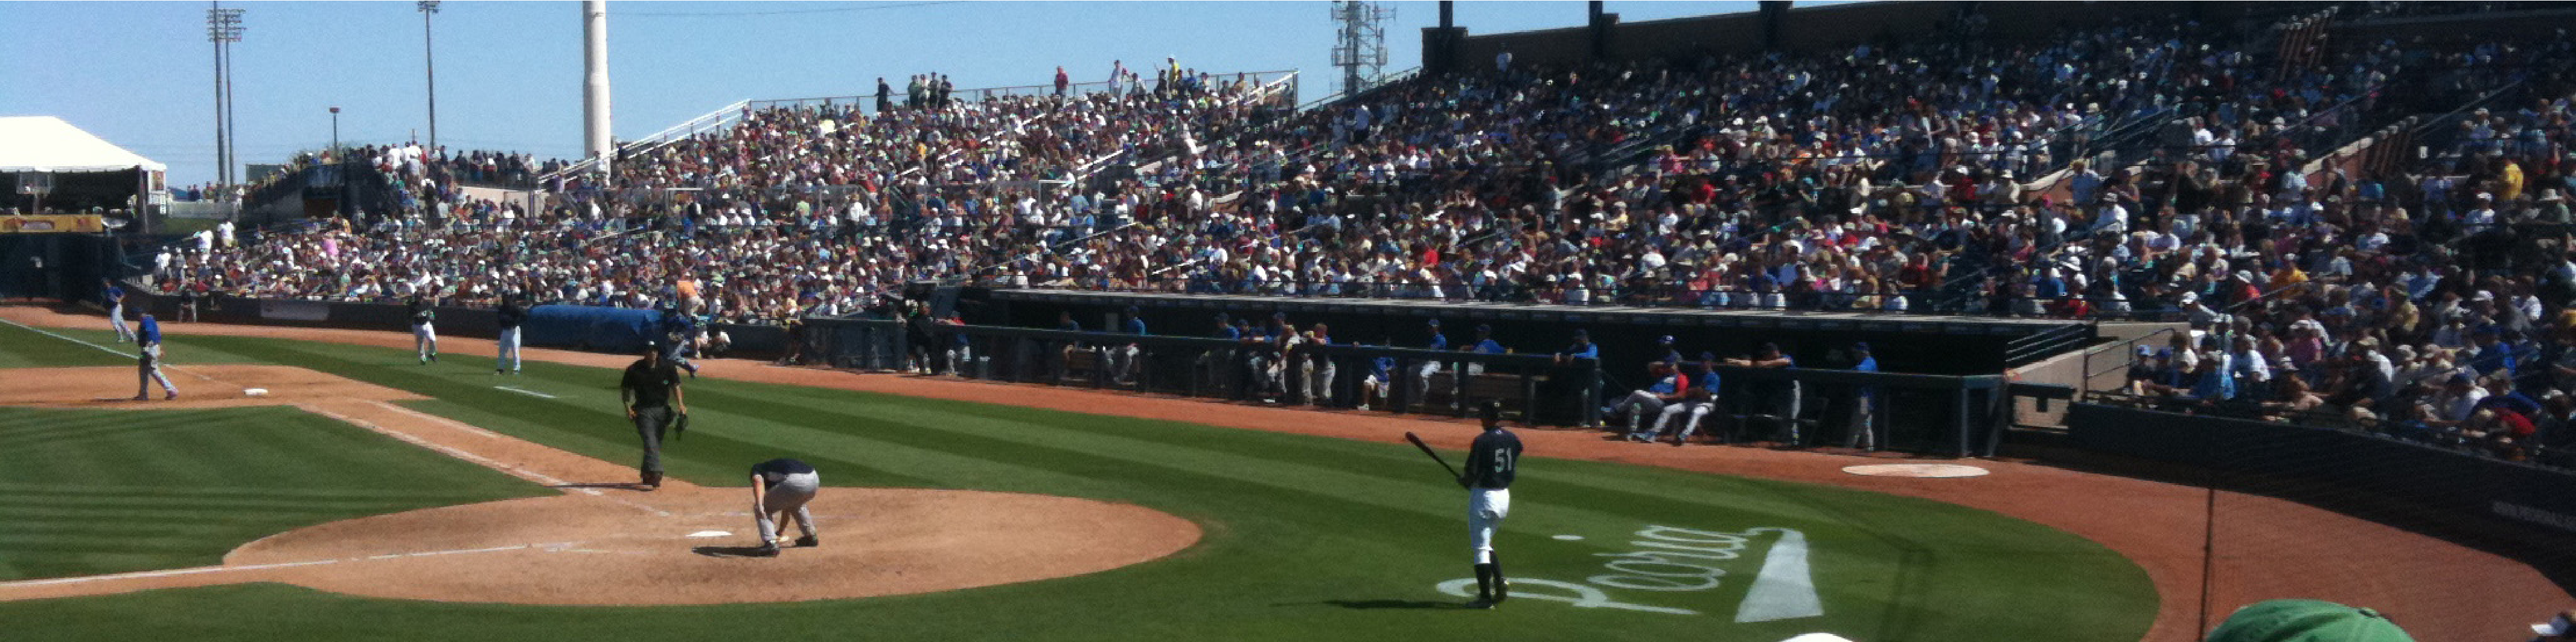
\includegraphics[width=\textwidth]{sampleteaser}
		\caption{Seattle Mariners at Spring Training, 2010.}
		\Description{Enjoying the baseball game from the third-base
			seats. Ichiro Suzuki preparing to bat.}
		\label{fig:teaser}
	\end{teaserfigure}
\fi

%%
%% This command processes the author and affiliation and title
%% information and builds the first part of the formatted document.
\maketitle

\section{Introduction}
In software development, code coverage is a critical metric that provides insight into the extent to which source code is tested, helping to identify untested areas and enhancing overall code quality. Traditional code coverage tools require a program to be fully executable, meaning they are unable to analyze incomplete or partially developed code. This requirement limits their utility during iterative development stages, where obtaining coverage feedback early in the process could be valuable in guiding subsequent coding and testing efforts.

Recent advancements in large language models (LLMs) offer a promising alternative for addressing these limitations. By leveraging natural language processing capabilities, LLMs can analyze code structure and semantics to estimate code coverage, even in the absence of compilation or execution. This potential makes LLMs especially useful for providing insights into coverage for partial programs, thereby supporting developers in assessing and improving coverage throughout the development process.

Our study extends prior work in this area, specifically building upon Codepilot, a prompt-crafting technique that explored code coverage estimation through LLMs for a single programming language. In Codepilot, LLMs were evaluated using a combination of few-shot, one-shot, and zero-shot prompting techniques, as well as different phases of query structuring. The two-phase approach involved generating a natural language plan for code coverage in the first phase, then feeding the plan back into the LLM to retrieve the actual coverage. The single-phase approach directly prompted the LLM to generate both the plan and the coverage in a single prompt. Codepilot identified the few-shot one-phase method as achieving the best results, suggesting that a single, context-rich prompt could effectively guide the LLM in understanding the code and estimating its coverage.

Expanding on these findings, our study applies the few-shot, one-phase prompting technique to a broader set of programming languages, encompassing five paradigms to investigate the adaptability and robustness of LLM-driven code coverage estimation. Specifically, we examine languages from functional, procedural, object-oriented, logic-based, and scripting paradigms: Haskell, C, Java, Prolog, and Python, respectively. Each language presents unique syntactic and semantic characteristics that represent the diverse ways in which code structures and logic are expressed in programming. By testing the few-shot prompting method across languages of varied paradigms, we aim to evaluate how well LLMs can generalize across programming styles, potentially extending the applicability of LLM-based code coverage to a wide range of software development environments.

This study is motivated by the growing demand for flexible tools that can aid developers working in multi-paradigm environments, where traditional coverage tools may not be consistently effective or available. In particular, understanding the performance of LLMs in handling coverage for diverse languages could inform their use in real-world settings where developers often encounter multiple paradigms within a single project. Our research aims to uncover insights into the strengths and limitations of LLMs as tools for cross-language code coverage and to contribute to the body of knowledge on LLM applications in software engineering. By demonstrating the potential for LLMs to provide coverage feedback for programs that are incomplete or non-executable, we hope to support the development of tools that enhance software quality and reduce risks associated with untested code across programming paradigms.

\section{Functional Programming}
Functional programming is a paradigm that emphasizes computation through the evaluation of functions and avoids changing states or mutable data. In this paradigm, programs are structured around the application of mathematical functions, where each function takes an input and returns a new value without altering any existing data. Haskell, a prominent functional language, embodies these principles with features like pure functions, immutability, and lazy evaluation (i.e., values are computed only when needed). This paradigm is known for its high level of abstraction and expressiveness, making it suitable for complex computations and enabling more predictable, side-effect-free code. Haskell’s functional characteristics allow for concise and expressive code, but these features can be challenging for conventional testing and code coverage tools to interpret due to the lack of mutable states and traditional control flow.

\section{Procedural Programming}
Procedural programming is a paradigm based on the concept of procedure calls, where a program is structured as a sequence of steps or instructions. It relies on routines, such as functions or subroutines, to perform tasks, and it emphasizes a clear, step-by-step structure that progresses through control flows like loops and conditionals. C is one of the most widely used procedural languages, offering low-level memory access and efficient execution. It is often favored in systems programming and applications requiring fine-grained control over hardware. Code in C is typically organized through procedures that manipulate data in variables, making code execution straightforward but sometimes complex in terms of tracking memory usage and managing pointer operations. Code coverage in procedural languages generally focuses on line or statement coverage, as well as function and branch coverage.

\section{Object-Oriented Programming}
Object-oriented programming (OOP) is centered around the concept of “objects”—data structures that combine data fields with methods for operating on the data. This paradigm promotes modularity and reusability by organizing code into classes and objects, each representing an instance of a class. Java is a quintessential object-oriented language that encapsulates data and methods within classes, using principles like inheritance, polymorphism, and encapsulation to model real-world entities and relationships. OOP facilitates code reuse, flexibility, and maintainability, making it popular in large-scale software development. However, the interconnected nature of objects and class hierarchies introduces additional complexity for code coverage, as tests must account for interactions among objects and potential inheritance chains that influence behavior across classes.

\section{Logic Programming}
Logic programming is a paradigm based on formal logic, where programs consist of a set of rules and facts. Computation in logic programming occurs through pattern matching and logical inference rather than sequential execution. Prolog, the primary language in this paradigm, uses a declarative approach in which problems are defined by relationships (facts) and rules, and the program searches for solutions that satisfy these logical constraints. This paradigm is well-suited to tasks in artificial intelligence and complex problem-solving, where solutions are derived through logical reasoning. In Prolog, code coverage involves evaluating how effectively rules and facts are tested, which can differ significantly from coverage metrics in imperative languages. Due to Prolog’s declarative nature, coverage analysis focuses on ensuring that logical paths and rule conditions are adequately exercised.

\section{Scripting and Dynamic Programming}
Scripting languages, often dynamically typed, focus on automating tasks and performing higher-level operations. Python, a popular scripting language, supports multiple programming paradigms, including procedural, functional, and object-oriented styles, offering flexibility in writing code. Python is dynamically typed, meaning that data types are inferred at runtime, which allows rapid development but can introduce runtime uncertainties. Its versatility and ease of use make Python a favored choice in fields such as data analysis, web development, and machine learning. Code coverage in Python often involves testing code paths and ensuring that dynamic features like runtime type inference and exception handling are adequately covered. The language’s dynamic nature and support for multiple paradigms present unique challenges for comprehensive coverage analysis, especially in understanding the interactions between different programming styles within the same codebase.

\section{Assessing CodePilot's Breadth}
Introduce our own work, and the motivation behind it, by talking about the fact that CodePilot is very new and has only been tested with Python, so very limited. Here we want to explore the breadth of CodePilot by testing it on different types of programming languages. We are interested in assessing both the quality of the plan that the model outputs, the quality of the code coverage prediction that the model outputs, and the link between the two (i.e. does it look like the model uses its own plan to predict code coverage). These are our research questions.

\section{Methodology}
Five different programming languages, each belonging to a different type of language class. Onephase. Two-shot, so we give two exemplars to the model. Two tests for each language. We match the exemplar and test language. We wanted small exemplars with some level of complexity. The two exemplars for all languages are implementations of the same algorithm, one with a certain level of complexity. The two tests for all languages are implementations of the same algorithm, one with a certain level of complexity. Talk about the exact algorithms. We run each experiment once. Temperature of 0.6. GPT instruct 3.5. The template that we use (the same as in CodePilot's original paper).

\begin{figure}[h]
	\centering
	\frame{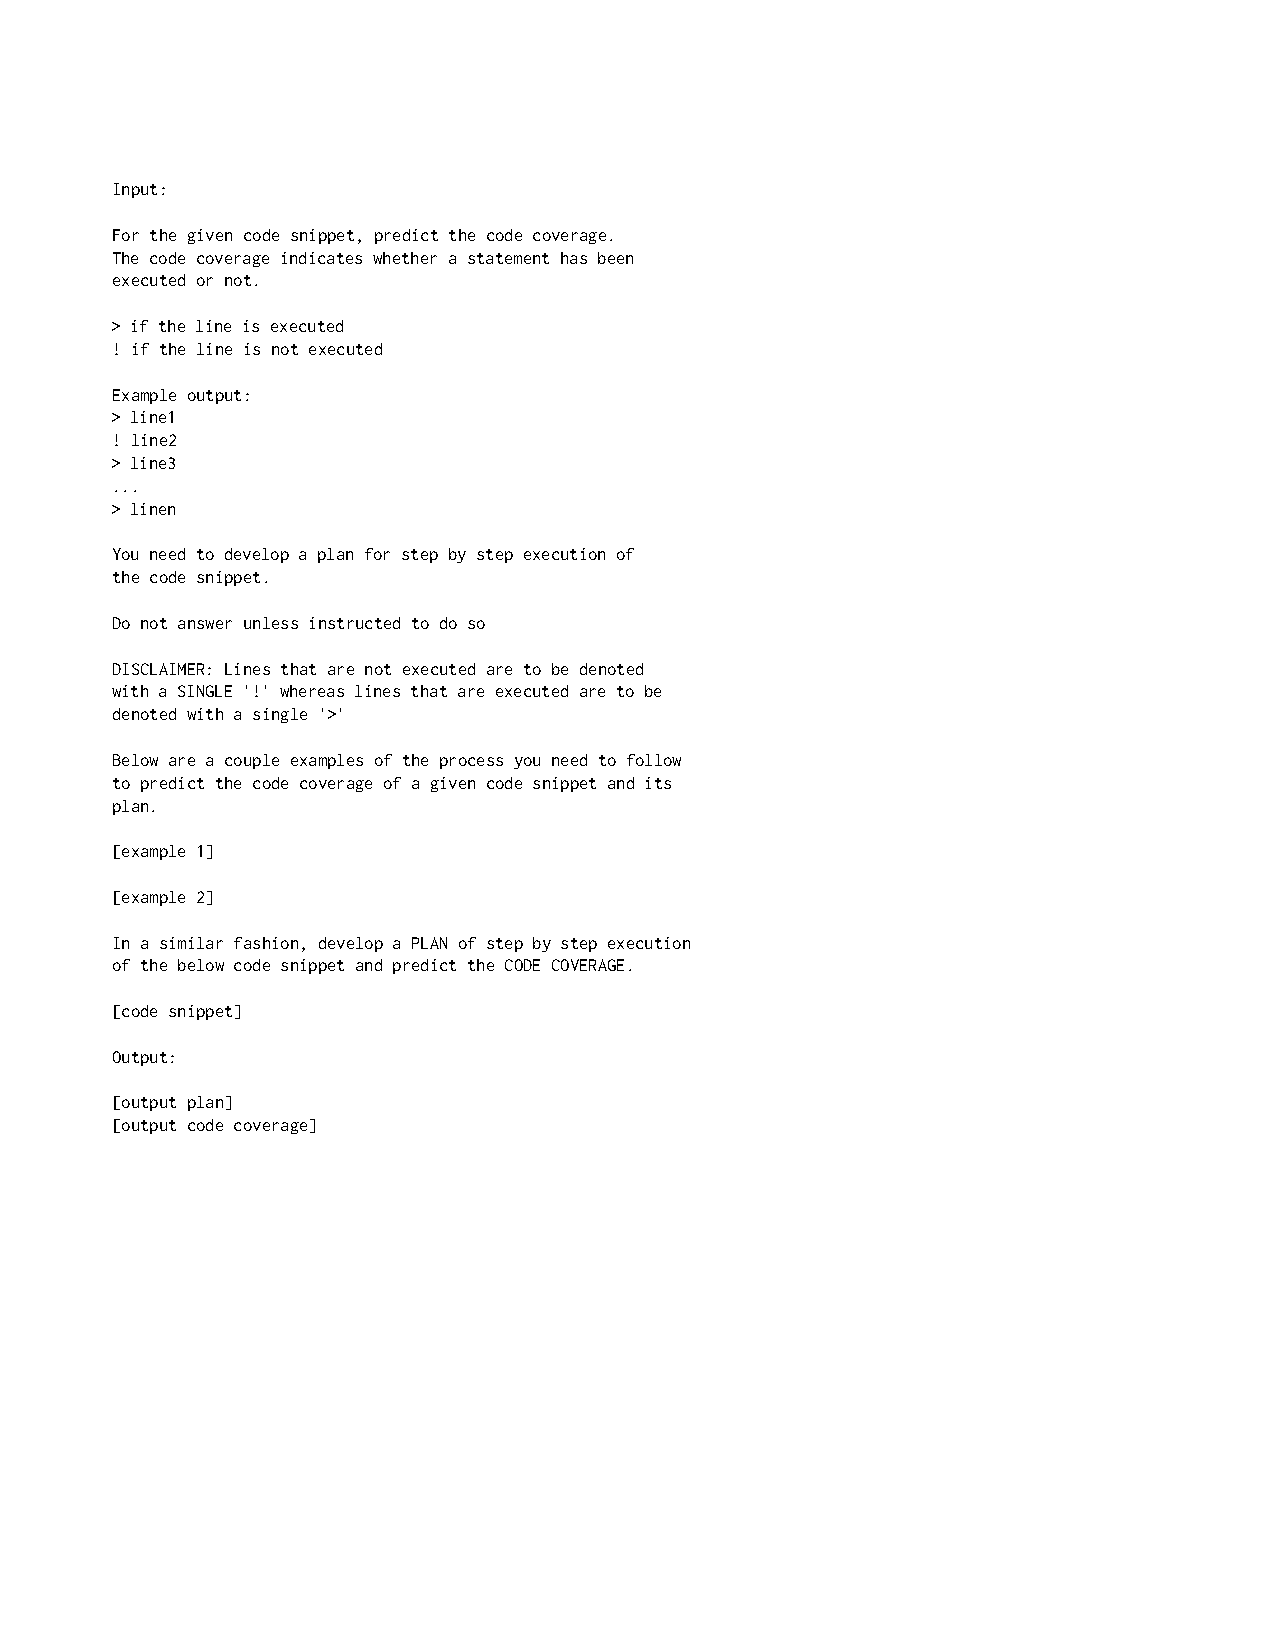
\includegraphics[width=\linewidth]{template_figure_final.pdf}}
	\caption{Template}
	\Description{template}
\end{figure}

Nam id fermentum dui. Suspendisse sagittis tortor a nulla mollis, in
pulvinar ex pretium. Sed interdum orci quis metus euismod, et sagittis
enim maximus. Vestibulum gravida massa ut felis suscipit
congue. Quisque mattis elit a risus ultrices commodo venenatis eget
dui. Etiam sagittis eleifend elementum.

\begin{figure}[h]
	\centering
	\frame{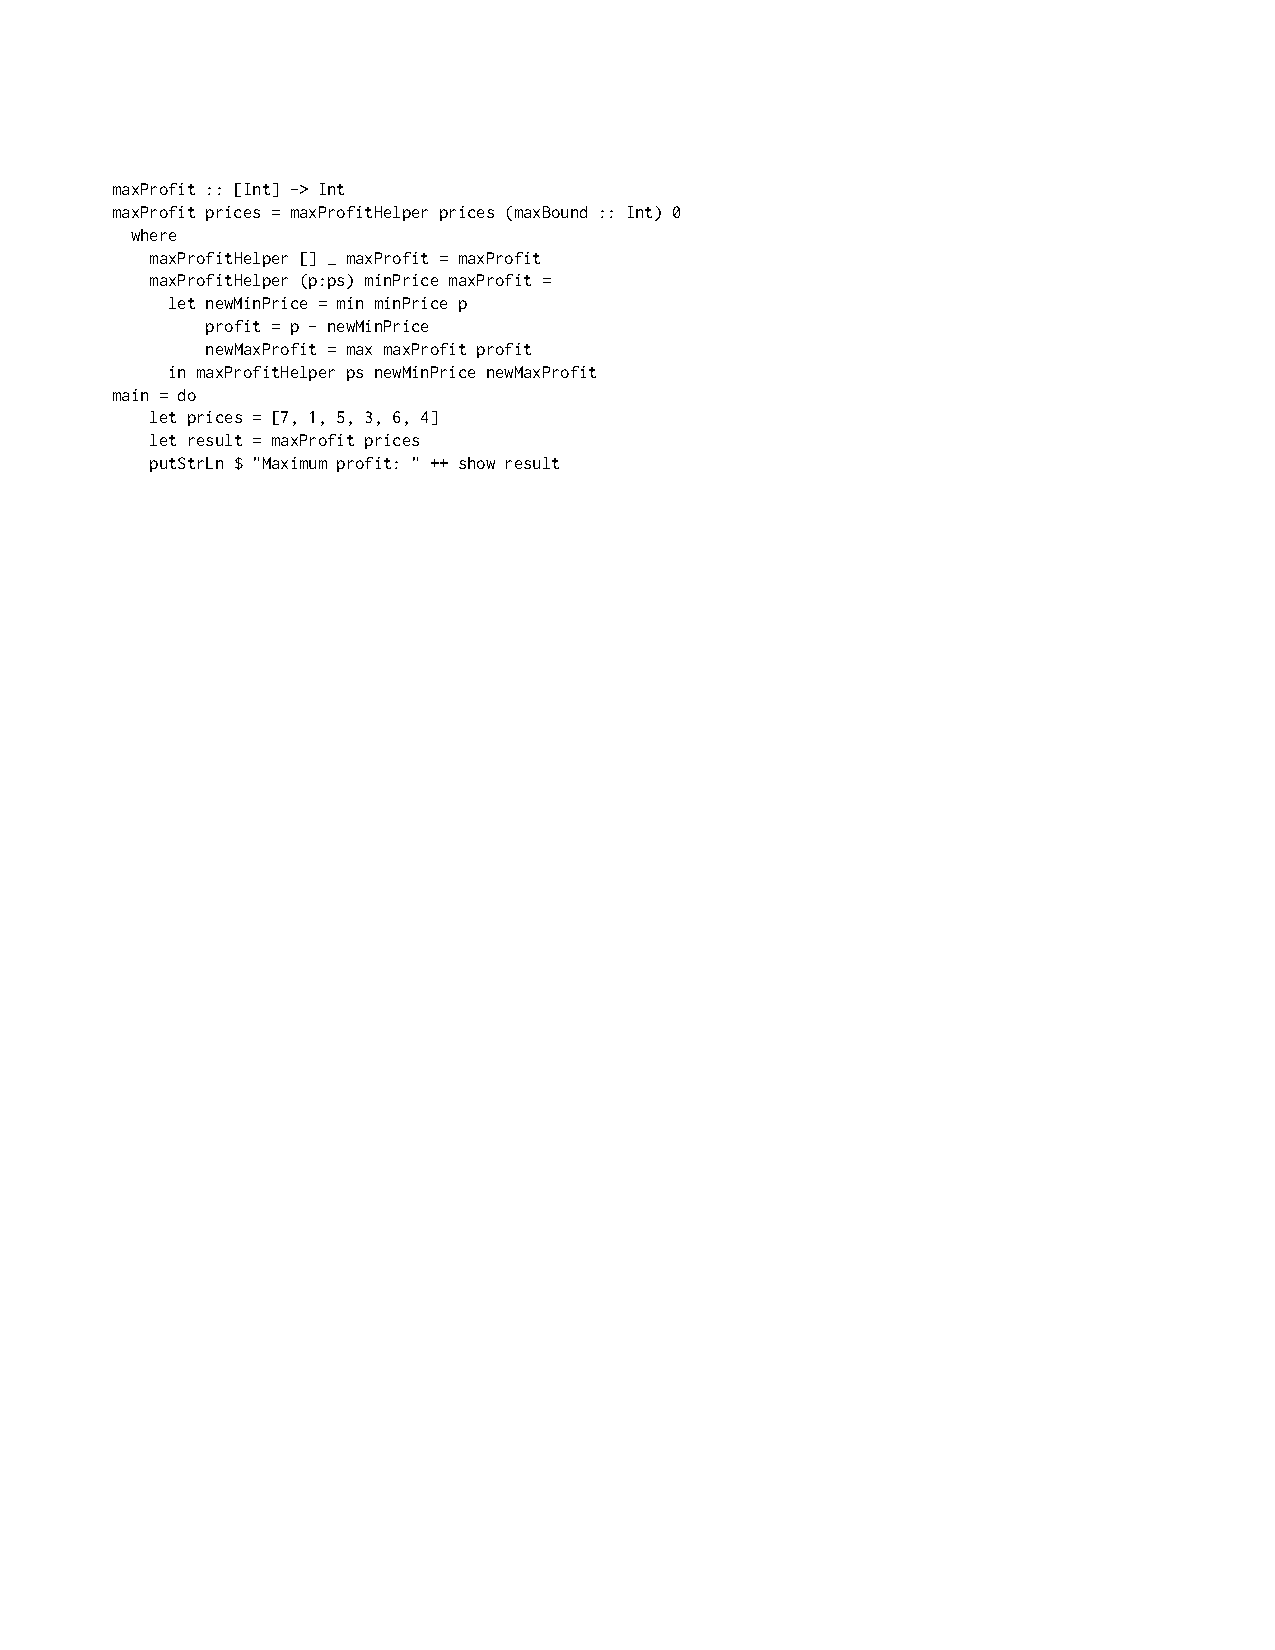
\includegraphics[width=\linewidth]{test_figure_final.pdf}}
	\caption{Test}
	\Description{test}
\end{figure}

Nam id fermentum dui. Suspendisse sagittis tortor a nulla mollis, in
pulvinar ex pretium. Sed interdum orci quis metus euismod, et sagittis
enim maximus. Vestibulum gravida massa ut felis suscipit
congue. Quisque mattis elit a risus ultrices commodo venenatis eget
dui. Etiam sagittis eleifend elementum.

\begin{figure}[h]
	\centering
	\frame{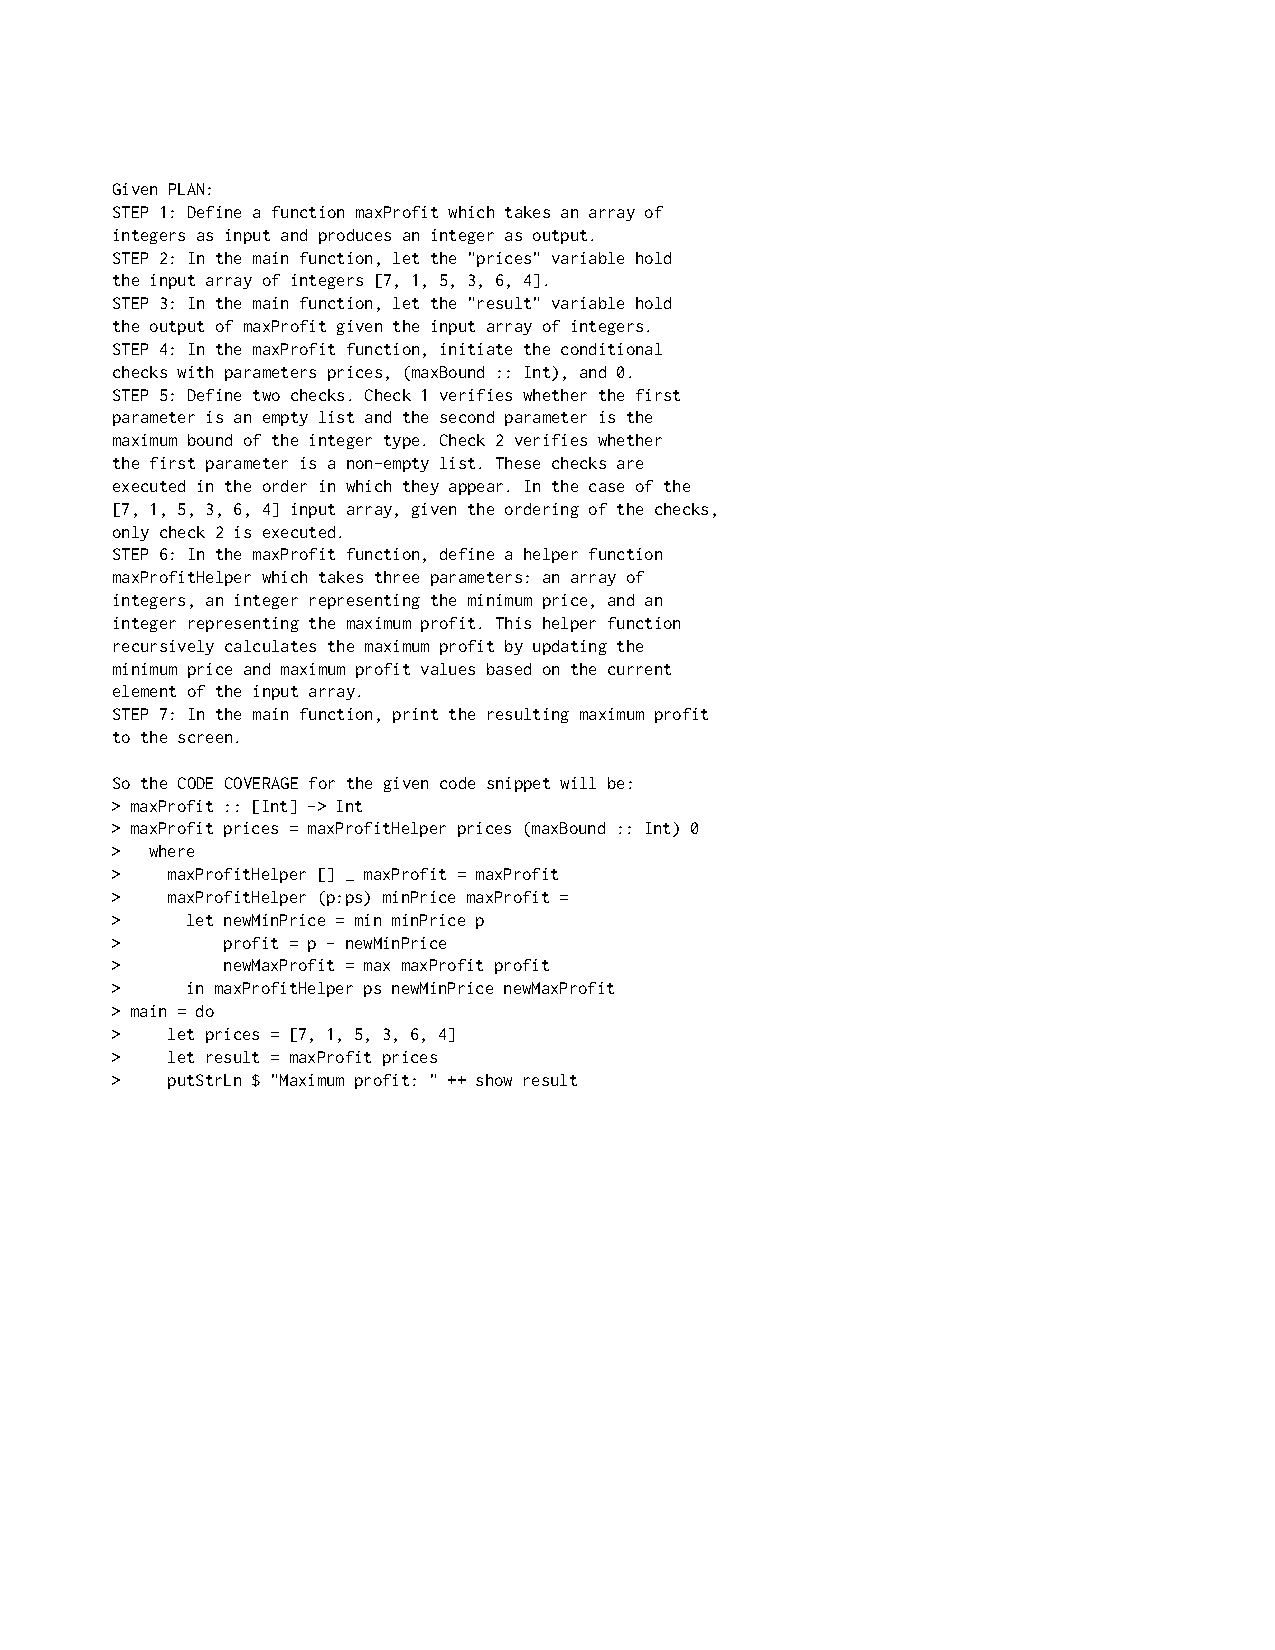
\includegraphics[width=\linewidth]{output_figure_final.pdf}}
	\caption{Output}
	\Description{output}
\end{figure}

Nam id fermentum dui. Suspendisse sagittis tortor a nulla mollis, in
pulvinar ex pretium. Sed interdum orci quis metus euismod, et sagittis
enim maximus. Vestibulum gravida massa ut felis suscipit
congue. Quisque mattis elit a risus ultrices commodo venenatis eget
dui. Etiam sagittis eleifend elementum.

\begin{figure}[h]
	\centering
	\frame{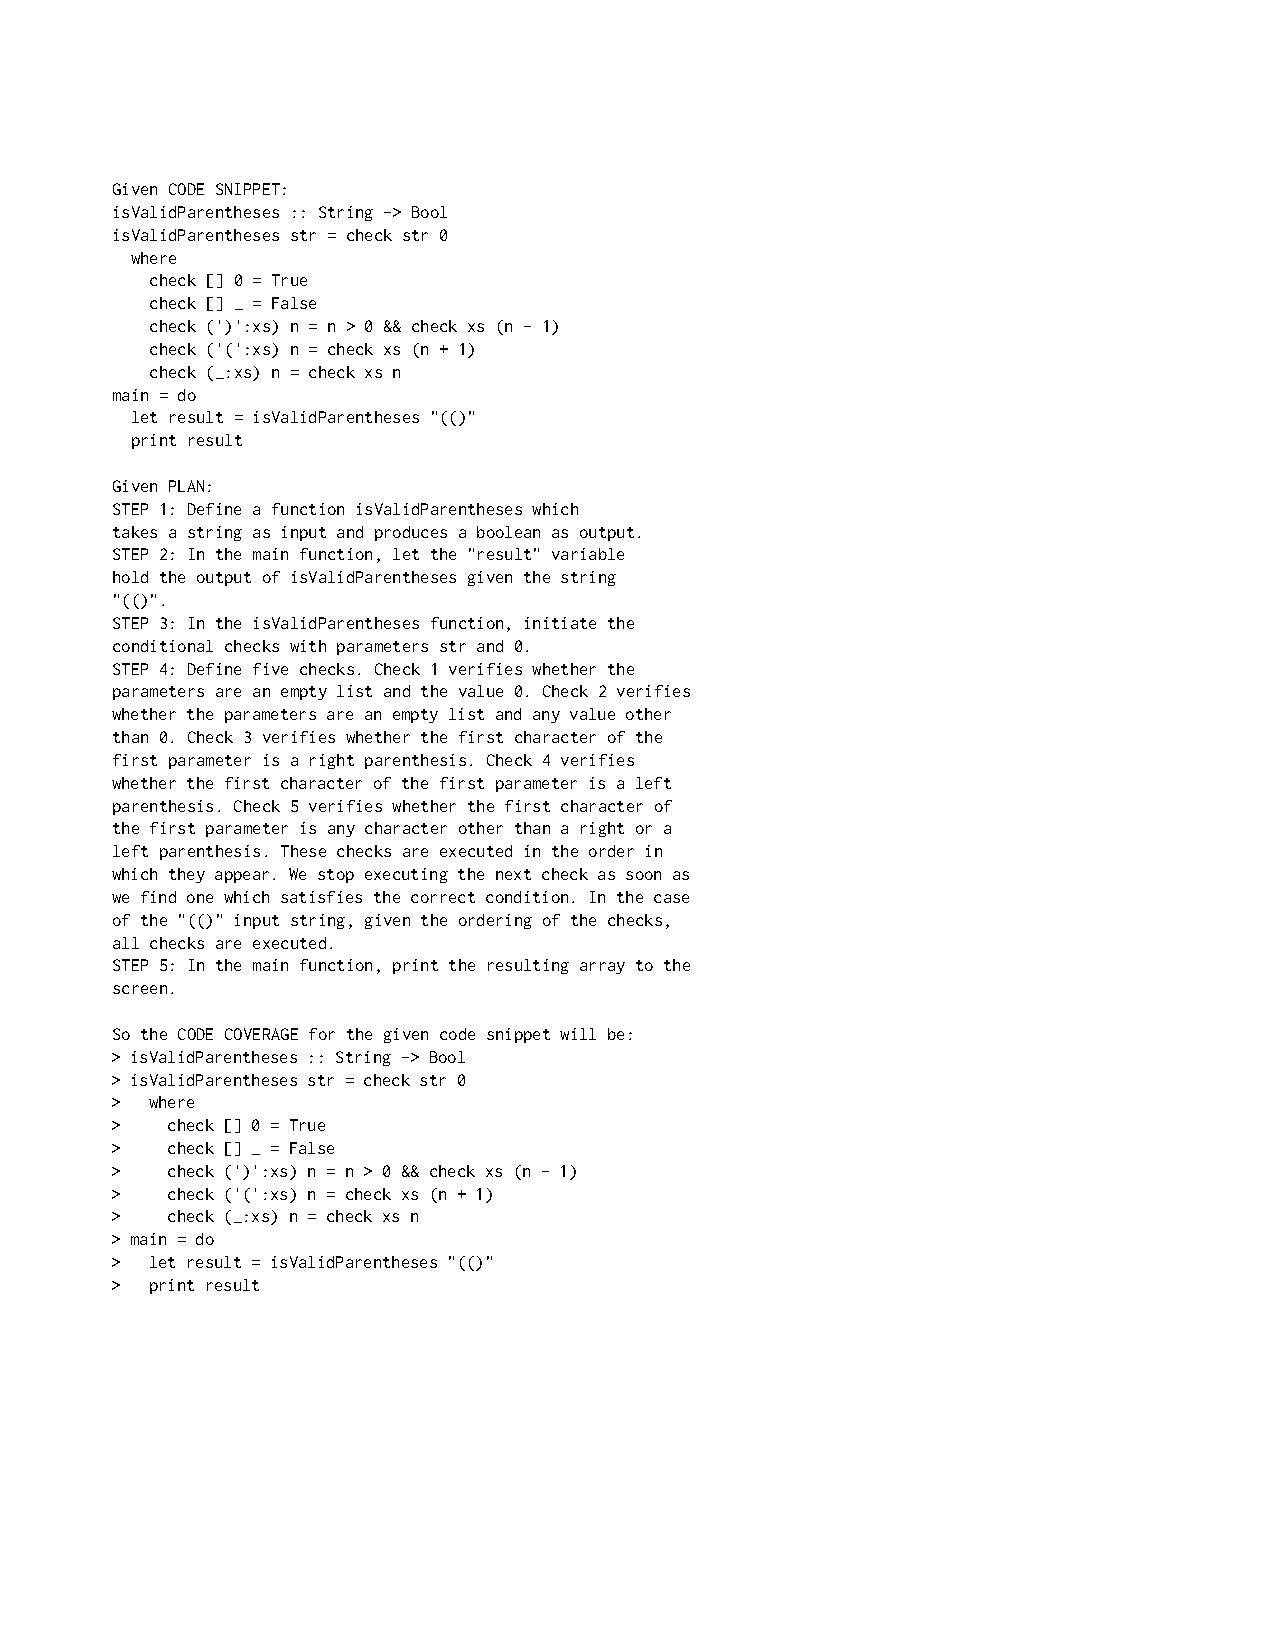
\includegraphics[width=\linewidth]{exemplar_figure_final.pdf}}
	\caption{Exemplar}
	\Description{exemplar}
\end{figure}

Nam id fermentum dui. Suspendisse sagittis tortor a nulla mollis, in
pulvinar ex pretium. Sed interdum orci quis metus euismod, et sagittis
enim maximus. Vestibulum gravida massa ut felis suscipit
congue. Quisque mattis elit a risus ultrices commodo venenatis eget
dui. Etiam sagittis eleifend elementum.

\section{Threats to Validity}
In any empirical study involving machine learning models, particularly large language models (LLMs), certain threats to validity may impact the reliability and generalizability of the findings. This study’s exploration of LLM-driven code coverage across multiple programming paradigms faces several specific challenges, outlined below. One major threat to validity is the non-deterministic nature of LLMs. Due to the stochastic nature of LLMs, the same prompt may yield different outputs across multiple runs. This characteristic introduces variability in the code coverage results generated by the LLM, which could impact the consistency of coverage estimates. This variability presents a challenge in replicating results and verifying the reliability of the coverage analysis across programming languages. Although our study uses a few-shot, one-phase prompting method, which has been shown to yield more consistent outputs than zero-shot approaches, there remains a risk that minor fluctuations in output may lead to inconsistencies in coverage analysis, particularly across languages with vastly different syntax and structure. Another potential threat is prompt sensitivity, the results generated by LLMs are highly sensitive to prompt construction, which can influence the accuracy and quality of the code coverage estimations. Minor modifications to prompts can produce significant changes in LLM responses, potentially affecting the results’ validity. In this study, we apply a carefully designed few-shot prompting technique; however, prompt engineering remains an inherently subjective process. The prompts used in our study might not generalize to other types of code or languages, limiting the applicability of our findings. Additionally, as prompt engineering evolves, new techniques may emerge that produce different results, posing a potential threat to the study’s replicability.

\section{Mitigation}
To address these threats, we have standardized prompt templates and experimented with prompt refinement to minimize variability. Additionally, by using a few-shot, one-phase prompting approach, we aim to reduce inconsistencies across runs, as this method has demonstrated higher stability than zero-shot or multi-phase alternatives. However, we acknowledge that the inherent variability of LLMs limits the extent to which these mitigations can fully eliminate the outlined threats.

\section{Future Directions}
This study represents an initial exploration into the use of large language models (LLMs) for code coverage estimation across multiple programming languages and paradigms. Given the scope and limitations of our current research design, several potential extensions could further enrich the findings and address the limitations noted. In our current study, we used only two examples in our few-shot prompting approach, which provided minimal context for the LLM. A natural extension would be to increase the number of examples to further ground the LLM's understanding of code coverage expectations. Adding more examples across diverse programming constructs and paradigms could improve the accuracy and reliability of coverage estimations, as a broader context may help the LLM generalize better to new, unseen code snippets. This could include examples featuring more complex control flows, various levels of nesting, and different algorithmic structures within each programming language. Additionally, experimenting with multi-shot prompts could allow us to analyze how many examples are optimal for consistent coverage estimations across paradigms.

Our current analysis focused on simple, isolated code snippets to test the feasibility of LLM-driven coverage estimation. Extending the study to encompass more complex, real-world codebases—such as multi-module applications or scripts with extensive dependencies—would present a valuable next step. By evaluating the LLM’s performance on these larger and more representative code samples, we could better assess the model’s applicability to practical software development scenarios. Testing on complex programs would also allow for the exploration of how well the LLM handles dependencies, external libraries, and interactions between modules.

Given the inherent non-determinism of LLMs, running multiple trials for each code snippet would allow us to observe and document the variability in coverage estimations. By collecting and analyzing a distribution of coverage outputs for each snippet, we could assess the stability and reliability of LLM-driven code coverage. Plotting this distribution would provide insights into the consistency of the model’s estimations and allow us to determine whether certain programming paradigms or language features result in higher variability. This extension could contribute valuable data for understanding how often LLMs yield inconsistent results and how best to mitigate this variability in practical applications.

Another valuable extension would involve benchmarking LLM-driven coverage against traditional code coverage tools (e.g., coverage.py, gcov) in multi-language, real-world applications. By comparing the coverage metrics generated by LLMs with those from execution-based tools, particularly on large codebases with mixed-paradigm languages, we could assess the feasibility of LLMs as a viable alternative to traditional coverage methods. This comparison would highlight the advantages and limitations of using LLMs in practical scenarios, identifying cases where LLMs might complement or substitute traditional tools, especially in early development stages.

Since LLMs are capable of handling multiple programming languages within the same prompt context, an extension of this study could focus on how well LLMs generalize code coverage techniques across paradigms in more nuanced ways. For instance, testing the LLM’s ability to transfer knowledge of code coverage patterns from one language (e.g., Python) to another (e.g., Prolog) could provide insights into its cross-language adaptability. This extension would be particularly useful in evaluating whether the LLM can consistently apply code coverage logic across different paradigms or if paradigm-specific adjustments are necessary.

\section{Results and Discussion}
Achieved results, and our interpretation of them.

\section{Conclusion and Future Directions}
Summary of main contributions. Why this study matters, how can our findings be used. Generally speaking we see that prompt and exemplar engineering is necessary in the sense that it really has an impact on the model's output, and they must be tailored to the specific task, the specific language.

\iffalse
	Modifying the template --- including but not limited to: adjusting
	margins, typeface sizes, line spacing, paragraph and list definitions,
	and the use of the \verb|\vspace| command to manually adjust the
	vertical spacing between elements of your work --- is not allowed.

	\section{Title Information}

	The title of your work should use capital letters appropriately -
	\url{https://capitalizemytitle.com/} has useful rules for
	capitalization. Use the {\verb|title|} command to define the title of
	your work. If your work has a subtitle, define it with the
		{\verb|subtitle|} command.  Do not insert line breaks in your title.

	If your title is lengthy, you must define a short version to be used
	in the page headers, to prevent overlapping text. The \verb|title|
	command has a ``short title'' parameter:
	\begin{verbatim}
  \title[short title]{full title}
\end{verbatim}

	\section{Sectioning Commands}

	Your work should use standard \LaTeX\ sectioning commands:
	\verb|section|, \verb|subsection|, \verb|subsubsection|, and
	\verb|paragraph|. They should be numbered; do not remove the numbering
	from the commands.

	\section{Tables}

	The ``\verb|acmart|'' document class includes the ``\verb|booktabs|''
	package --- \url{https://ctan.org/pkg/booktabs} --- for preparing
	high-quality tables.

	Table captions are placed {\itshape above} the table.

	Because tables cannot be split across pages, the best placement for
	them is typically the top of the page nearest their initial cite.  To
	ensure this proper ``floating'' placement of tables, use the
	environment \textbf{table} to enclose the table's contents and the
	table caption.  The contents of the table itself must go in the
	\textbf{tabular} environment, to be aligned properly in rows and
	columns, with the desired horizontal and vertical rules.  Again,
	detailed instructions on \textbf{tabular} material are found in the
	\textit{\LaTeX\ User's Guide}.

	Immediately following this sentence is the point at which
	Table~\ref{tab:freq} is included in the input file; compare the
	placement of the table here with the table in the printed output of
	this document.

	\begin{table}
		\caption{Frequency of Special Characters}
		\label{tab:freq}
		\begin{tabular}{ccl}
			\toprule
			Non-English or Math & Frequency   & Comments          \\
			\midrule
			\O                  & 1 in 1,000  & For Swedish names \\
			$\pi$               & 1 in 5      & Common in math    \\
			\$                  & 4 in 5      & Used in business  \\
			$\Psi^2_1$          & 1 in 40,000 & Unexplained usage \\
			\bottomrule
		\end{tabular}
	\end{table}

	To set a wider table, which takes up the whole width of the page's
	live area, use the environment \textbf{table*} to enclose the table's
	contents and the table caption.  As with a single-column table, this
	wide table will ``float'' to a location deemed more
	desirable. Immediately following this sentence is the point at which
	Table~\ref{tab:commands} is included in the input file; again, it is
	instructive to compare the placement of the table here with the table
	in the printed output of this document.

	\begin{table*}
		\caption{Some Typical Commands}
		\label{tab:commands}
		\begin{tabular}{ccl}
			\toprule
			Command                    & A Number & Comments         \\
			\midrule
			\texttt{{\char'134}author} & 100      & Author           \\
			\texttt{{\char'134}table}  & 300      & For tables       \\
			\texttt{{\char'134}table*} & 400      & For wider tables \\
			\bottomrule
		\end{tabular}
	\end{table*}

	Always use midrule to separate table header rows from data rows, and
	use it only for this purpose. This enables assistive technologies to
	recognise table headers and support their users in navigating tables
	more easily.

	\section{Math Equations}
	You may want to display math equations in three distinct styles:
	inline, numbered or non-numbered display.  Each of the three are
	discussed in the next sections.

	\subsection{Inline (In-text) Equations}
	A formula that appears in the running text is called an inline or
	in-text formula.  It is produced by the \textbf{math} environment,
	which can be invoked with the usual
	\texttt{{\char'134}begin\,\ldots{\char'134}end} construction or with
	the short form \texttt{\$\,\ldots\$}. You can use any of the symbols
	and structures, from $\alpha$ to $\omega$, available in
	\LaTeX~\cite{Lamport:LaTeX}; this section will simply show a few
	examples of in-text equations in context. Notice how this equation:
	\begin{math}
		\lim_{n\rightarrow \infty}x=0
	\end{math},
	set here in in-line math style, looks slightly different when
	set in display style.  (See next section).

	\subsection{Display Equations}
	A numbered display equation---one set off by vertical space from the
	text and centered horizontally---is produced by the \textbf{equation}
	environment. An unnumbered display equation is produced by the
	\textbf{displaymath} environment.

	Again, in either environment, you can use any of the symbols and
	structures available in \LaTeX\@; this section will just give a couple
	of examples of display equations in context.  First, consider the
	equation, shown as an inline equation above:
	\begin{equation}
		\lim_{n\rightarrow \infty}x=0
	\end{equation}
	Notice how it is formatted somewhat differently in
	the \textbf{displaymath}
	environment.  Now, we'll enter an unnumbered equation:
	\begin{displaymath}
		\sum_{i=0}^{\infty} x + 1
	\end{displaymath}
	and follow it with another numbered equation:
	\begin{equation}
		\sum_{i=0}^{\infty}x_i=\int_{0}^{\pi+2} f
	\end{equation}
	just to demonstrate \LaTeX's able handling of numbering.

	\section{Citations and Bibliographies}

	The use of \BibTeX\ for the preparation and formatting of one's
	references is strongly recommended. Authors' names should be complete
	--- use full first names (``Donald E. Knuth'') not initials
	(``D. E. Knuth'') --- and the salient identifying features of a
	reference should be included: title, year, volume, number, pages,
	article DOI, etc.

	The bibliography is included in your source document with these two
	commands, placed just before the \verb|\end{document}| command:
	\begin{verbatim}
  \bibliographystyle{ACM-Reference-Format}
  \bibliography{bibfile}
\end{verbatim}
	where ``\verb|bibfile|'' is the name, without the ``\verb|.bib|''
	suffix, of the \BibTeX\ file.

	Citations and references are numbered by default. A small number of
	ACM publications have citations and references formatted in the
	``author year'' style; for these exceptions, please include this
	command in the {\bfseries preamble} (before the command
	``\verb|\begin{document}|'') of your \LaTeX\ source:
	\begin{verbatim}
  \citestyle{acmauthoryear}
\end{verbatim}


	Some examples.  A paginated journal article \cite{Abril07}, an
	enumerated journal article \cite{Cohen07}, a reference to an entire
	issue \cite{JCohen96}, a monograph (whole book) \cite{Kosiur01}, a
	monograph/whole book in a series (see 2a in spec. document)
	\cite{Harel79}, a divisible-book such as an anthology or compilation
	\cite{Editor00} followed by the same example, however we only output
	the series if the volume number is given \cite{Editor00a} (so
	Editor00a's series should NOT be present since it has no vol. no.),
	a chapter in a divisible book \cite{Spector90}, a chapter in a
	divisible book in a series \cite{Douglass98}, a multi-volume work as
	book \cite{Knuth97}, a couple of articles in a proceedings (of a
	conference, symposium, workshop for example) (paginated proceedings
	article) \cite{Andler79, Hagerup1993}, a proceedings article with
	all possible elements \cite{Smith10}, an example of an enumerated
	proceedings article \cite{VanGundy07}, an informally published work
	\cite{Harel78}, a couple of preprints \cite{Bornmann2019,
		AnzarootPBM14}, a doctoral dissertation \cite{Clarkson85}, a
	master's thesis: \cite{anisi03}, an online document / world wide web
	resource \cite{Thornburg01, Ablamowicz07, Poker06}, a video game
	(Case 1) \cite{Obama08} and (Case 2) \cite{Novak03} and \cite{Lee05}
	and (Case 3) a patent \cite{JoeScientist001}, work accepted for
	publication \cite{rous08}, 'YYYYb'-test for prolific author
	\cite{SaeediMEJ10} and \cite{SaeediJETC10}. Other cites might
	contain 'duplicate' DOI and URLs (some SIAM articles)
	\cite{Kirschmer:2010:AEI:1958016.1958018}. Boris / Barbara Beeton:
	multi-volume works as books \cite{MR781536} and \cite{MR781537}. A
	couple of citations with DOIs:
	\cite{2004:ITE:1009386.1010128,Kirschmer:2010:AEI:1958016.1958018}. Online
	citations: \cite{TUGInstmem, Thornburg01, CTANacmart}.
	Artifacts: \cite{R} and \cite{UMassCitations}.

	%%
	%% The acknowledgments section is defined using the "acks" environment
	%% (and NOT an unnumbered section). This ensures the proper
	%% identification of the section in the article metadata, and the
	%% consistent spelling of the heading.

	\begin{acks}
		To Robert, for the bagels and explaining CMYK and color spaces.
	\end{acks}

	%%
	%% The next two lines define the bibliography style to be used, and
	%% the bibliography file.
	\bibliographystyle{ACM-Reference-Format}
	\bibliography{sample-base}


	%%
	%% If your work has an appendix, this is the place to put it.
	\appendix

	\section{Appendix}

	\subsection{Part One}
	...

	\subsection{Part Two}
	...

	\newpage
	\section{Notes}
	\begin{verbatim}
Input:

For the given code snippet, predict the code coverage.
The code coverage indicates whether a statement has been
executed or not.

> if the line is executed
! if the line is not executed

Example output:
> line1
! line2
> line3
...
> linen

You need to develop a plan for step by step execution of
the code snippet.

Do not answer unless instructed to do so

DISCLAIMER: Lines that are not executed are to be denoted
with a SINGLE '!' whereas lines that are executed are to be
denoted with a single '>'

Below are a couple examples of the process you need to follow
to predict the code coverage of a given code snippet and its
plan.

[example 1]

[example 2]

In a similar fashion, develop a PLAN of step by step execution
of the below code snippet and predict the CODE COVERAGE.

[code snippet]

Output:

[output plan]
[output code coverage]

\end{verbatim}

	\newpage
	%exemplar
	\begin{verbatim}
Given CODE SNIPPET:
isValidParentheses :: String -> Bool
isValidParentheses str = check str 0
  where
    check [] 0 = True
    check [] _ = False
    check (')':xs) n = n > 0 && check xs (n - 1)
    check ('(':xs) n = check xs (n + 1)
    check (_:xs) n = check xs n
main = do
  let result = isValidParentheses "(()"
  print result

Given PLAN: 
STEP 1: Define a function isValidParentheses which
takes a string as input and produces a boolean as output.
STEP 2: In the main function, let the "result" variable
hold the output of isValidParentheses given the string
"(()".
STEP 3: In the isValidParentheses function, initiate the
conditional checks with parameters str and 0.
STEP 4: Define five checks. Check 1 verifies whether the
parameters are an empty list and the value 0. Check 2 verifies
whether the parameters are an empty list and any value other
than 0. Check 3 verifies whether the first character of the
first parameter is a right parenthesis. Check 4 verifies
whether the first character of the first parameter is a left
parenthesis. Check 5 verifies whether the first character of
the first parameter is any character other than a right or a
left parenthesis. These checks are executed in the order in
which they appear. We stop executing the next check as soon as
we find one which satisfies the correct condition. In the case
of the "(()" input string, given the ordering of the checks,
all checks are executed.
STEP 5: In the main function, print the resulting array to the
screen.

So the CODE COVERAGE for the given code snippet will be: 
> isValidParentheses :: String -> Bool
> isValidParentheses str = check str 0
>   where
>     check [] 0 = True
>     check [] _ = False
>     check (')':xs) n = n > 0 && check xs (n - 1)
>     check ('(':xs) n = check xs (n + 1)
>     check (_:xs) n = check xs n
> main = do
>   let result = isValidParentheses "(()"
>   print result
\end{verbatim}

	%test
	\begin{verbatim}
maxProfit :: [Int] -> Int
maxProfit prices = maxProfitHelper prices (maxBound :: Int) 0
  where
    maxProfitHelper [] _ maxProfit = maxProfit
    maxProfitHelper (p:ps) minPrice maxProfit =
      let newMinPrice = min minPrice p
          profit = p - newMinPrice
          newMaxProfit = max maxProfit profit
      in maxProfitHelper ps newMinPrice newMaxProfit
main = do
    let prices = [7, 1, 5, 3, 6, 4]
    let result = maxProfit prices
    putStrLn $ "Maximum profit: " ++ show result
\end{verbatim}

	%output
	\begin{verbatim}
Given PLAN:
STEP 1: Define a function maxProfit which takes an array of
integers as input and produces an integer as output.
STEP 2: In the main function, let the "prices" variable hold
the input array of integers [7, 1, 5, 3, 6, 4].
STEP 3: In the main function, let the "result" variable hold
the output of maxProfit given the input array of integers.
STEP 4: In the maxProfit function, initiate the conditional
checks with parameters prices, (maxBound :: Int), and 0.
STEP 5: Define two checks. Check 1 verifies whether the first
parameter is an empty list and the second parameter is the
maximum bound of the integer type. Check 2 verifies whether
the first parameter is a non-empty list. These checks are
executed in the order in which they appear. In the case of the
[7, 1, 5, 3, 6, 4] input array, given the ordering of the checks,
only check 2 is executed.
STEP 6: In the maxProfit function, define a helper function
maxProfitHelper which takes three parameters: an array of
integers, an integer representing the minimum price, and an
integer representing the maximum profit. This helper function
recursively calculates the maximum profit by updating the
minimum price and maximum profit values based on the current
element of the input array.
STEP 7: In the main function, print the resulting maximum profit
to the screen.

So the CODE COVERAGE for the given code snippet will be: 
> maxProfit :: [Int] -> Int
> maxProfit prices = maxProfitHelper prices (maxBound :: Int) 0
>   where
>     maxProfitHelper [] _ maxProfit = maxProfit
>     maxProfitHelper (p:ps) minPrice maxProfit =
>       let newMinPrice = min minPrice p
>           profit = p - newMinPrice
>           newMaxProfit = max maxProfit profit
>       in maxProfitHelper ps newMinPrice newMaxProfit
> main = do
>     let prices = [7, 1, 5, 3, 6, 4]
>     let result = maxProfit prices
>     putStrLn $ "Maximum profit: " ++ show result
\end{verbatim}
\fi

\end{document}
\endinput
%%
%% End of file `sample-sigconf.tex'.
